
\chapter{Einführung}
\label{sec:intro}
	Dieses Kapitel soll einen Überblick über Motivation, Ziel sowie Struktur der vorliegenden Arbeit verschaffen. Außerdem wird ein theoretisches Basiswissen in den Bereichen Bildverarbeitung und Evolutionäre Algorithmen bereitgestellt, welches notwendig ist, um den Kontext dieses Erzeugnisses greifbar zu machen. 
		
	\section{Grundlegendes über Bildverarbeitung}
	\label{sec:bild-basics}
		
		In den zurückliegenden Textpassagen dieses Schriftstücks wurde die Bildverarbeitung bereits mehrfach erwähnt - aber was ist das denn konkret? Tatsächlich gibt es hier keine einheitliche Definition - das liegt unter anderem daran, dass die Grenzen zwischen Bildverarbeitung und maschinellem Sehen nicht klar abgesteckt werden können. Eine mögliche Definition wird von Rafael C. Gonzalez und Richard E. Woods in ihrem Buch \textit{Digital Image Processing} \cite{gonzalez-woods-imgproc} beschrieben. Hierzu nehmen sie zunächst eine Unterscheidung von rechnergestützten Prozessen wie folgt vor: 
		\begin{description}
			\item[Low-Level] Darunter fallen einfache Operationen direkt am Bild, wie zum Beispiel Rauschreduktion oder die Erhöhung des Kontrastes. Input sowie Output sind jeweils durch ein Bild gegeben.
			\item[Mid-Level] Diese Kategorie von Prozessen zeichnet sich dadurch aus, dass aus einem Bild bestimmte Eigenschaften/Bereiche extrahiert werden, um daraus eine Information zu gewinnen. Exemplarisch hierfür kann die Segmentierung angeführt werden, die im Rahmen dieser Arbeit als Versuchsobjekt für den in Abschnitt \ref{sec:de} vorgestellten Algorithmus dient. Während der Input aus einem ganzen Bild besteht, beläuft sich der Output lediglich auf einen Teil davon beziehungsweise ein bestimmtes Attribut des Bildes.
			\item[High-Level] Hier werden die aus den Mid-Level Prozessen erhaltenen Informationen verwendet, um bestimmte Aktionen auszulösen (z.B. im Bezug auf maschinelles Sehen)
		\end{description}
		
		Auf dieser Grundlage definieren die Autoren in \cite{gonzalez-woods-imgproc} den Terminus der Bildverarbeitung als Menge aller Low- und Mid-Level Prozesse. \\
		
		Einen in der heutigen Zeit zentralen Anwendungsfall für die Bildverarbeitung stellt \gls{ocr} dar. Wie der Name bereits vermuten lässt, ist das Ziel der \gls{ocr}, Zeichen oder Formen aus digitalen Bildern zu extrahieren und weiterzuverarbeiten. Schon in den frühen 1950ern - so bei \cite{cher-et-al-ocr} - haben Forscher nach Möglichkeiten gesucht, auf Papier befindlichen Text rechnergestützt einzulesen, um dem Menschen die mühselige Arbeit des manuellen Abtippens von Dokumenten abzunehmen. Abbildung \ref{fig:ocr-system} illustriert hierbei die Vorgänge in einem typischen System, das \gls{ocr} realisieren soll. 
		
		\begin{figure}[H]
			\centering
			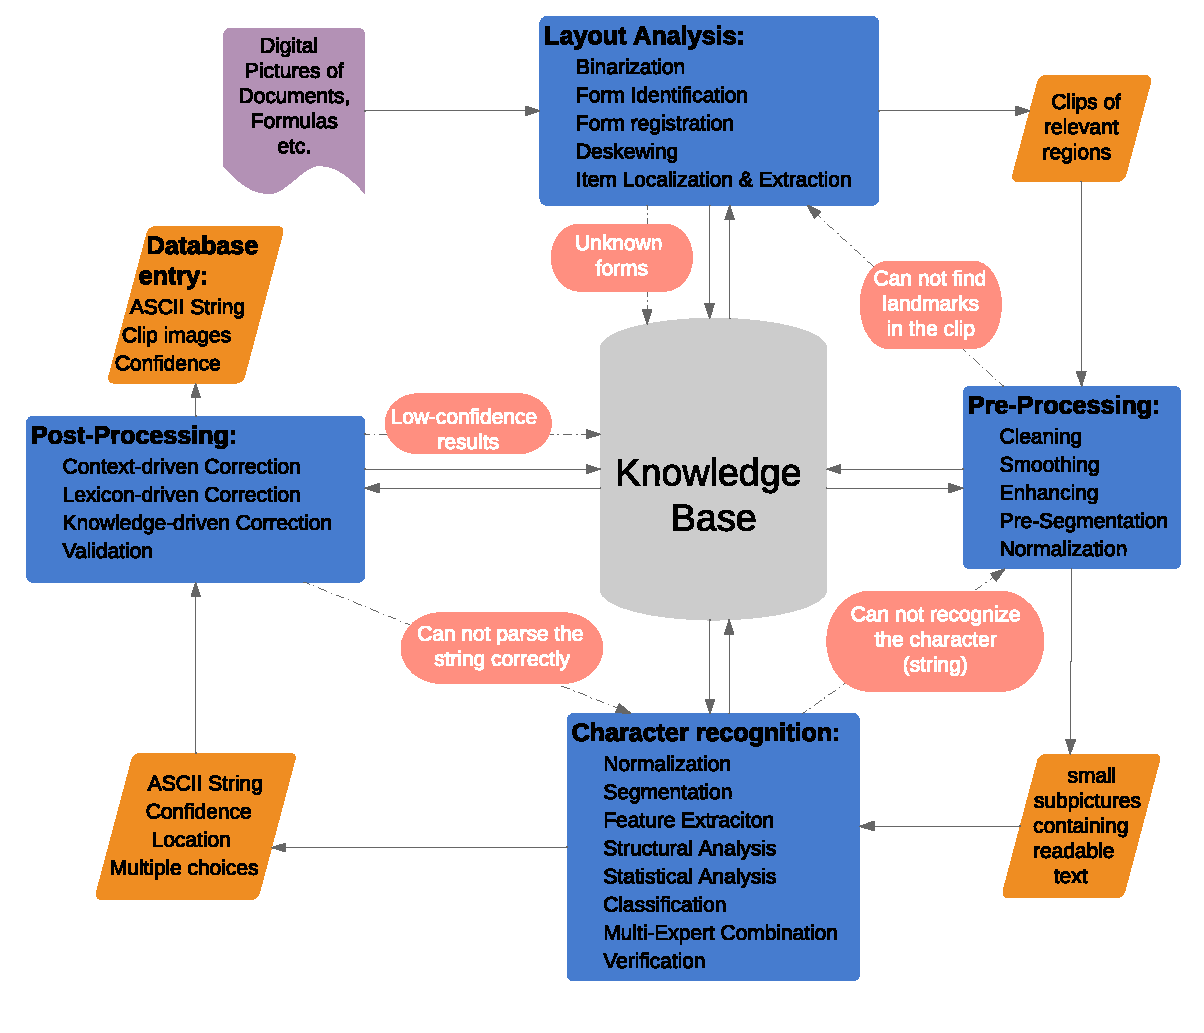
\includegraphics[width=0.7\linewidth]{Ablauf-OCR_Cheriet-et-al}
			\caption[typisches \gls{ocr}-Ablaufschema]{Schematische Darstellung des Ablaufs in einem intelligenten \gls{ocr}-System (aus \cite{cher-et-al-ocr})}
			\label{fig:ocr-system}
		\end{figure}
		
	\glsreset{ea}
	
	\section{\gls{ea}}
	\label{sec:evol}
		
		In der September-Ausgabe des Magazins \textit{Spektrum der Wissenschaft} \cite{j-h-holland} aus dem Jahr 1992 ließen sich folgende Worte von John H. Holland lesen: \\
		
		\begin{quote}
			\textit{Lebewesen sind vollendete Problemlöser. In der Vielzahl der Aufgaben, die sie bewältigen, übertreffen sie die besten Computerprogramme bei weitem - zur besonderen Frustration der Programmierer, die Monate oder gar Jahre harter geistiger Arbeit für einen Algorithmus aufwenden, während Organismen ihre Fähigkeiten durch den scheinbar ziellosen Mechanismus der Evolution erwerben. \\}
		\end{quote}
		
		Dieses Zitat, welches die Einleitung von \cite{ger-kla-kru-intro} bildet, bietet bereits eine grobe Vorstellung vom Wesen und der Herkunft von \gls{ea}. In den meisten literarischen Werken zu diesem Thema - beispielsweise \cite{ger-kla-kru-intro}, \cite{eib-smi-ea} - wird festgehalten, dass verschiedene Kategorien von \gls{ea} existieren. Allerdings ist diese Einteilung laut \cite{eib-smi-ea} lediglich historischer Natur und verschwimmt zunehmend. Ursächlich hierfür ist, dass der einzige Unterschied zwischen den einzelnen Varianten in der Repräsentation\footnote{mögliche Darstellungsformen sind - wie in \cite{eib-smi-ea} beschrieben - Strings (\textbf{Genetische Algorithmen}), Vektoren von (reellen) Zahlen (\textbf{Evolutionsstrategien}) und Baumstrukturen (\textbf{Genetische Programmierung}) sowie endliche Automaten (\textbf{Evolutionäre Programmierung})} der Lösungskandidaten (hierzu in Kürze mehr) liegt. Die Funktionsweise, welche allen \gls{ea} zugrunde liegt, ist dieselbe: \\
		
		\begin{itemize}
			\item Gegeben sei eine Liste von Lösungskandidaten (im Folgenden \textbf{Population} genannt) als Input für eine Zielfunktion (fortlaufend als \textbf{Fitnessfunktion} bezeichnet), die in der Regel minimiert oder maximiert werden soll.
			\item Des weiteren sei diese Population von der Generation $n$.
			\item Zunächst wird die Fitness jener n-ten Population mithilfe der Fitnessfunktion ausgewertet und zwischengespeichert. 
			\item Aus dieser wird mittels verschiedener Variationsoperationen (\textbf{Rekombination}, \textbf{Mutation}) eine neue Population  erzeugt.
			\item Im nächsten Schritt wird diese ebenfalls durch die Fitnessfunktion evaluiert.
			\item Um anschließend eine Population der Generation $n+1$ zu generieren, deren Fitness größer gleich der $n$-ten Population ist, wird eine \textbf{Selektion}soperation durchgeführt, die aus den beiden vorliegenden Populationen jeweils die Kandidaten mit der besten Fitness auswählt.
		\end{itemize}
		
		Die soeben beschriebene Vorgehensweise kann so lange wiederholt werden, bis entweder eine gewünschte Lösung vorliegt oder ein (vorher festgelegtes) Iterationslimit erreicht ist. Im folgenden Abschnitt werden all diese Aspekte anhand eines Beispielalgorithmus, welcher ebenfalls im Rahmen dieser Arbeit verwendet wird, deutlich.\\
		
		
		%Im Buch \cite{eib-smi-ea} findet ebenfalls Erwähnung, dass es zwar 
		%eine Kategorisierung von \gls{ea}s gibt, diese jedoch lediglich 
		%historischer Natur ist und einzig auf der Repräsentation der 
		%Populationsmitglieder beruht. Beispielsweise werden sie bei den 
		%\textbf{Genetischen Algorithmen} als Strings dargestellt, während die 
		%\textbf{Evolutionsstrategien} diese als Vektoren von reellen Werten 
		%verarbeiten. In der Praxis wählt man ohnehin diejenige 
		%Darstellungsart, 
		%welche für die spezifische Anwendung am geeignetsten ist.
		
	\glsreset{de}
	
	\section{\gls{de}}
	\label{sec:de}
	
	\section{Ziel}
	\label{sec:ziel}
	
		Nun, nachdem der theoretische Grundstein gelegt wurde, lässt sich die Intention dieser Arbeit formulieren:
		\begin{itemize}
			\item Sie soll erstens die Problemstellung in einer klaren Form präsentieren (Abschnitt \ref{sec:motivation}) sowie in ein möglichst passendes mathematisches Modell unter Einbettung von \gls{de} übersetzen (Abschnitt \ref{sec:imp}).
			\item Zweitens wird eine Umsetzungsstrategie zur Implementierung dieses Modells beschrieben (Abschnitt \ref{sec:imp}).
			\item Schlussendlich sollen die Testergebnisse dieser Umsetzung in Kapitel \ref{sec:ex} veranschaulicht werden. Darauf aufbauend findet eine Bewertung hinsichtlich der Tauglichkeit der vorgestellten Strategie zur Lösung der eingangs in Abschnitt \ref{sec:motivation} geschilderten Problemstellung statt (Kapitel \ref{sec:sumary}). Zudem wird ein Ausblick auf mögliche Verbesserungsansätze geboten. 
		\end{itemize}
	
	\section{Motivation}
	\label{sec:motivation}